\documentclass[a4paper]{article}
\usepackage[polish]{babel}
\usepackage[T1]{fontenc}
\usepackage{graphicx}
\usepackage{float}
\usepackage{hyperref}
\usepackage{titling}
\predate{}
\postdate{}
\usepackage[left=2cm,right=2cm,top=0.1cm,bottom=2cm]{geometry}
\title{Dokumentacja\\ Drzewo Genealogiczne - Proof of concept}
\author{Mariusz Biegański}
\date{}
\begin{document}
\maketitle

\section{Wstęp}
Celem projektu jest wykorzystanie bazy danych Neo4j do zweryfikowania możliwości 
jej zastosowania do rozwiązania określonego problemu lub realizacji konkretnego 
celu. Implementacja pozwala zauważyć zarówno korzyści, jak i ewentualne 
ograniczenia związane z wykorzystaniem tej technologii w danym projekcie. 
Projek Proof of Concept ogranicza koszty przed wyborem technologii do 
projektu biznesowego.

\section{Funkcjonalność}
Aplikacja umożliwia następujące funkcjonalności:
\begin{itemize}
\item Przeglądanie listy osób zapisanych w bazie danych Neo4j oraz ich relacji.
\item Dodawanie nowych osób do bazy danych.
\item Aktualizowanie danych osoby zapisanej w bazie danych.
\item Usuwanie osób zapisanych w bazie danych.
\item Tworzenie nowych relacji między osobami zapisanymi w bazie danych.
\item Wyszukiwanie relacji między dwoma osobami zapisanymi w bazie danych.
\item Wizualizację relacji pomiędzy osobami
\end{itemize}

\section{Diagram UML}

\begin{figure}[H]
	\centering
	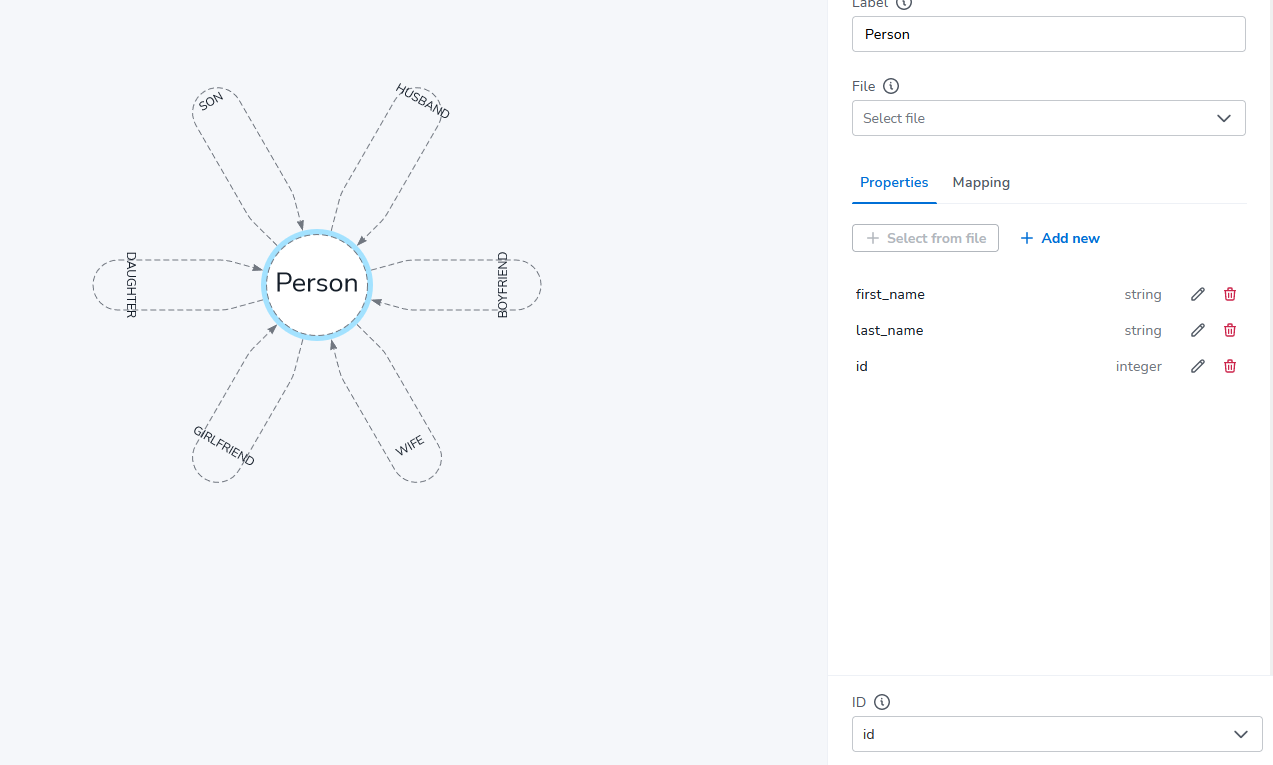
\includegraphics[width=\linewidth]{diagram.png}
	\caption{Diagram przedstawiający węzeł Person wraz z własnościami i relacjami}
\end{figure}

\section{Technologie}

Aplikacja wykorzystuje następujące technologie:
\begin{itemize}
\item \textbf{Neo4j}: grafowa baza danych służąca do przechowywania i przetwarzania danych w formie grafu.
\item \textbf{AuraDB}: darmowa usługa hostingowa dla bazy danych Neo4j
\item \textbf{Express.js}: framework sieciowy służący do obsługi żądań HTTP i tworzenia aplikacji sieciowych.
\item \textbf{EJS}: silnik szablonów umożliwiający wstawienie dynamicznych danych do szablonów stron internetowych.
\item \textbf{Vis.js}: biblioteka JavaScript do tworzenia interaktywnych wizualizacji danych i diagramów.
\item \textbf{Render}: darmowa usługa hostingowa umożliwiająca hostowanie aplikacji Node.js. Aplikacja jest dostępna pod adresem \href{https://family-tree-rq7c.onrender.com/}{https://family-tree-rq7c.onrender.com/}.
\end{itemize}

\section{Wdrożenie}
Do połączenia z bazą danych Neo4j został użyty moduł neo4j-driver. 
Adres bazy danych oraz dane do logowania są odczytywane z pliku credentials.env 
za pomocą modułu dotenv.

Aplikacja obsługuje różne żądania HTTP, takie jak GET i POST, które służą do 
pobierania danych lub przesyłania danych do bazy. Na przykład, żądanie GET '/' 
renderuje stronę główną aplikacji, która wyświetla przyciski nawigacyjne, 
listę osób i ich relacji z pobranymi danymi z bazy danych oraz wizualizuje dane. 
Żądanie POST '/new-person' dodaje nową osobę do bazy danych za pomocą przesłanych 
danych z formularza.

Aby pobrać dane z bazy danych, aplikacja wywołuje asynchroniczne funkcje, takie 
jak \texttt{get\_persons}, \texttt{get\_relations} i \texttt{get\_data}. 
Funkcje te wysyłają zapytania w języku Cypher do bazy danych, a następnie 
przetwarzają otrzymane dane, aby wyświetlić je na stronie.

Przy każdym żądaniu aplikacja pobiera nowe dane z bazy danych, aby zapewnić 
aktualność widoku. Dzięki temu użytkownik ma zawsze dostęp do najnowszych 
danych z bazy.

\section{Wnioski}

Baza danych Neo4j posiada następujące korzyści:

\begin{itemize}
\item Łatwe modelowanie i przechowywanie danych opartych na relacjach między elementami.
\item Możliwość wykonywania złożonych zapytań z wykorzystaniem języka Cypher.
\item Dobra integracja z innymi narzędziami oraz możliwość łatwego rozszerzenia 
	o nowe funkcjonalności.
\item Otwarta, rozwijająca się społeczność oraz szeroki wybór narzędzi i 
	bibliotek wspierających pracę z Neo4j.
\item Baza grafowa pozwala na lepsze zrozumienie powiązań między danymi, co może pomóc np.
	w ujawnieniu przestępstw czy innych nieprawidłowości
\end{itemize}

\end{document}
